\documentclass{article}
\usepackage{amsmath,amssymb}
\usepackage{graphicx}
\usepackage{enumerate}
\usepackage{hyperref}
\usepackage{subcaption}
\usepackage{caption}
\usepackage{xcolor}
\usepackage{float}

\pagestyle{empty} \addtolength{\textwidth}{1.0in}
\addtolength{\textheight}{0.5in}
\addtolength{\oddsidemargin}{-0.5in}
\addtolength{\evensidemargin}{-0.5in}
\newcommand{\ruleskip}{\bigskip\hrule\bigskip}
\newcommand{\nodify}[1]{{\sc #1}}
\newcommand{\points}[1]{{\textbf{[#1 points]}}}
\newcommand{\subquestionpoints}[1]{{[#1 points]}}
\newenvironment{answer}{{\bf Answer:} \sf }{}%

\newcommand{\bitem}{\begin{list}{$\bullet$}%
{\setlength{\itemsep}{0pt}\setlength{\topsep}{0pt}%
\setlength{\rightmargin}{0pt}}}
\newcommand{\eitem}{\end{list}}

\setlength{\parindent}{0pt} \setlength{\parskip}{0.5ex}
\setlength{\unitlength}{1cm}

\newcommand{\pa}[1]{[[PA: #1]]}

\renewcommand{\Re}{{\mathbb R}}
\newcommand{\E}{{\rm E}}
\begin{document}

\pagestyle{myheadings} \markboth{}{CS 294-158 Deep Unsupervised Learning, Homework 1, Spring 2024}

{\huge
\noindent Homework 1: Autoregressive Models}

\hfill \break
Name: Nolan Wagener
\ruleskip

{\bf Deliverable}: This PDF write-up by {\bf Tuesday February 7th, 23:59pm}.  Your PDF should be generated by simply replacing the placeholder images of this LaTeX document with the appropriate solution images that will be generated automatically when solving each question. The solution images are automatically generated and saved using the accompanying IPython notebook. Your PDF is to be submitted into Gradescope. This PDF already contains a few solution images.  These images will allow you to check your own solution to ensure correctness. Submit this PDF, your iPython notebook, and any other code you wrote to Gradescope!


\vspace{.2in}

%--------------------------------------------------------------------------------
%--------------------------------------------------------------------------------
%--------------------------------------------------------------------------------
\noindent {\bf Question 1: 1D Data}
%--------------------------------------------------------------------------------
%--------------------------------------------------------------------------------
%--------------------------------------------------------------------------------

\begin{enumerate}[(a)]

\item {\bf [10pt] Fitting a Histogram} \\\\
Final test loss for dataset 1: 2.548 nats/dim
\begin{figure}[H]
    \centering
    \begin{subfigure}{0.45\textwidth}
        \centering
        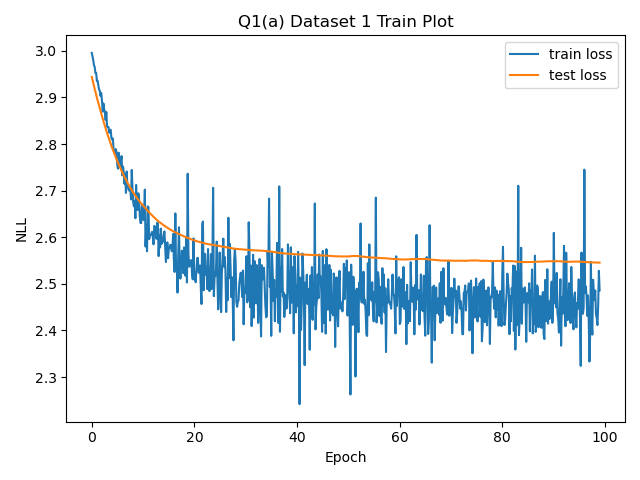
\includegraphics[width=\textwidth]{figures/q1_a_dset1_train_plot.png}
        \caption{Dataset 1: Training curve}
    \end{subfigure}
    \hspace{0.2in}
    \begin{subfigure}{0.45\textwidth}
        \centering
        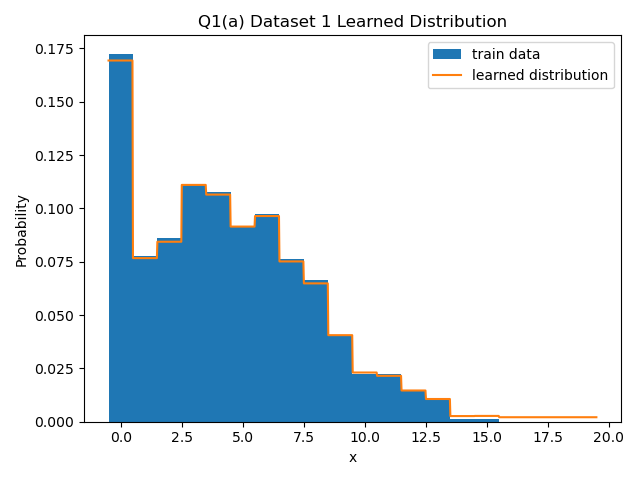
\includegraphics[width=\textwidth]{figures/q1_a_dset1_learned_dist.png}
        \caption{Dataset 1: Learned distribution}
    \end{subfigure}
\end{figure}
Final test loss for dataset 2: 3.686 nats/dim
\begin{figure}[H]
    \centering
    \begin{subfigure}{0.45\textwidth}
        \centering
        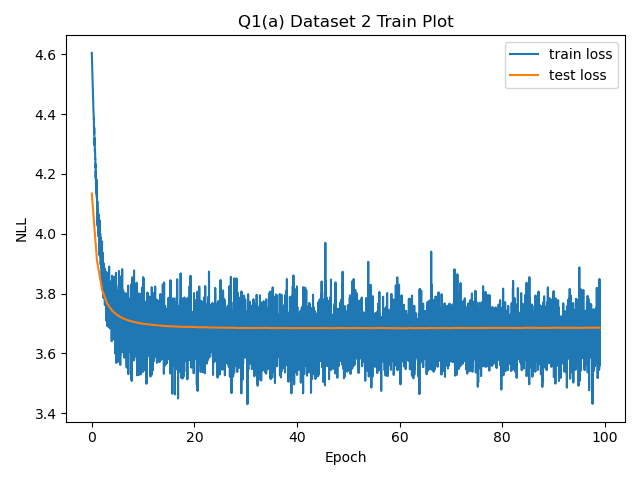
\includegraphics[width=\textwidth]{figures/q1_a_dset2_train_plot.png}
        \caption{Dataset 2: Training curve}
    \end{subfigure}
    \hspace{0.2in}
    \begin{subfigure}{0.45\textwidth}
        \centering
        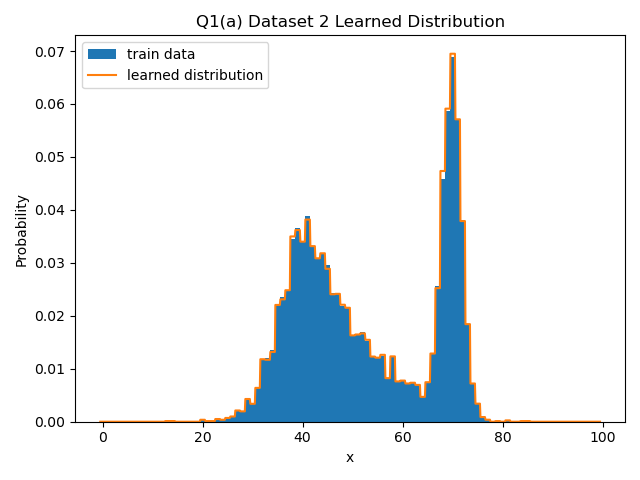
\includegraphics[width=\textwidth]{figures/q1_a_dset2_learned_dist.png}
        \caption{Dataset 2: Learned distribution}
    \end{subfigure}
\end{figure}

\newpage

\item {\bf [10pt] Fitting Discretized Mixture of Logistics} \\\\
Final test loss for dataset 1: 2.554 nats/dim
\begin{figure}[H]
    \centering
    \begin{subfigure}{0.45\textwidth}
        \centering
        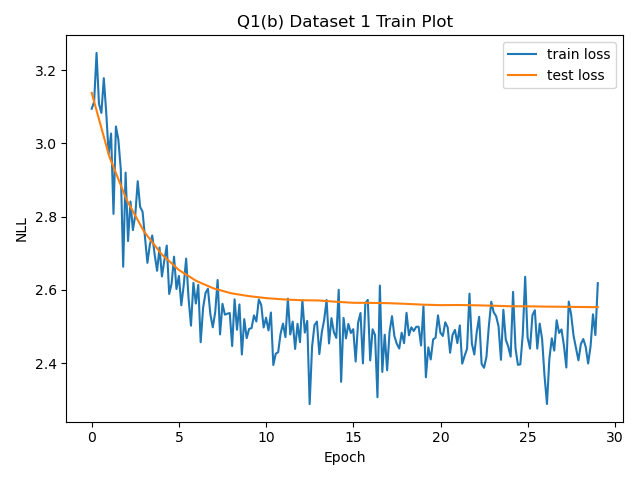
\includegraphics[width=\textwidth]{figures/q1_b_dset1_train_plot.png}
        \caption{Dataset 1: Training curve}
    \end{subfigure}
    \hspace{0.2in}
    \begin{subfigure}{0.45\textwidth}
        \centering
        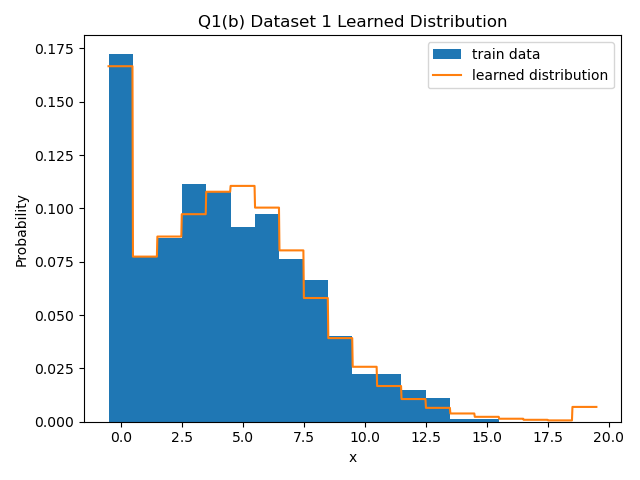
\includegraphics[width=\textwidth]{figures/q1_b_dset1_learned_dist.png}
        \caption{Dataset 1: Learned distribution}
    \end{subfigure}
\end{figure}
Final test loss for dataset 2: 3.717 nats/dim
\begin{figure}[H]
    \centering
    \begin{subfigure}{0.45\textwidth}
        \centering
        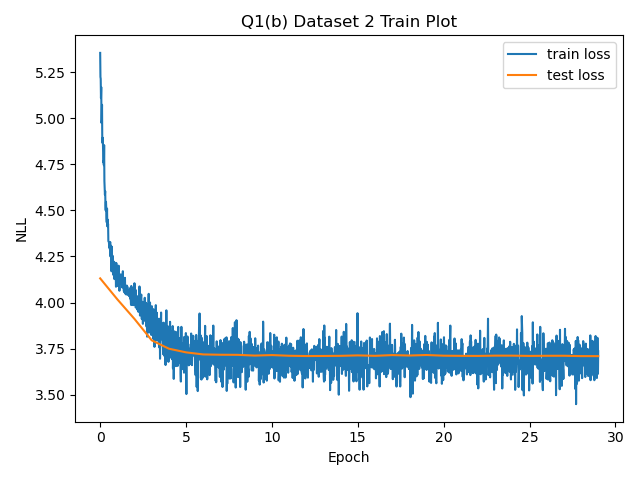
\includegraphics[width=\textwidth]{figures/q1_b_dset2_train_plot.png}
        \caption{Dataset 2: Training curve}
    \end{subfigure}
    \hspace{0.2in}
    \begin{subfigure}{0.45\textwidth}
        \centering
        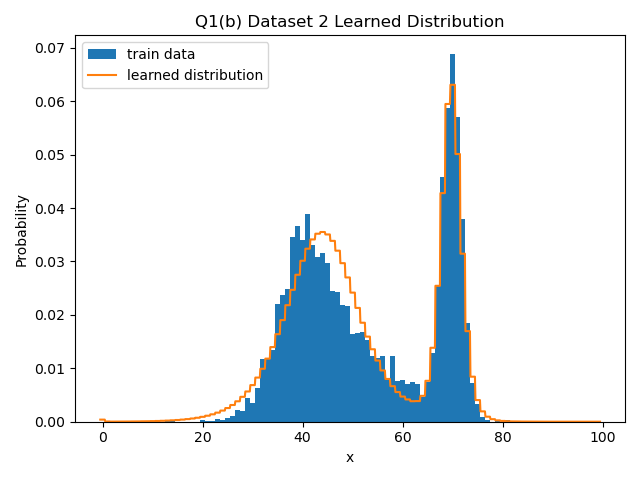
\includegraphics[width=\textwidth]{figures/q1_b_dset2_learned_dist.png}
        \caption{Dataset 2: Learned distribution}
    \end{subfigure}
\end{figure}
\end{enumerate}


%--------------------------------------------------------------------------------
%--------------------------------------------------------------------------------
%--------------------------------------------------------------------------------
\newpage
\noindent {\bf Question 2: PixelCNNs}
%--------------------------------------------------------------------------------
%--------------------------------------------------------------------------------
%--------------------------------------------------------------------------------

\begin{enumerate}[(a)]
\item {\bf [15pt] PixelCNNs on Shapes and MNIST} \\\\
Final test loss for dataset 1: 0.0429 nats/dim
\begin{figure}[H]
    \centering
    \begin{subfigure}{0.45\textwidth}
        \centering
        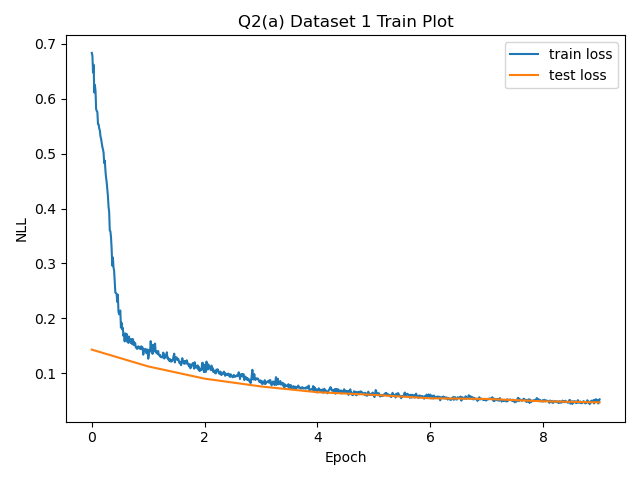
\includegraphics[width=\textwidth]{figures/q2_a_dset1_train_plot.png}
        \caption{Dataset 1: Training curve}
    \end{subfigure}
    \hspace{0.2in}
    \begin{subfigure}{0.45\textwidth}
        \centering
        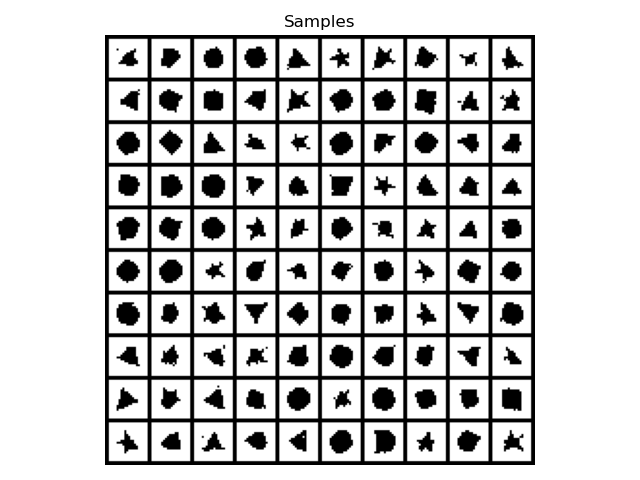
\includegraphics[width=\textwidth]{figures/q2_a_dset1_samples.png}
        \caption{Dataset 1: Samples}
    \end{subfigure}
\end{figure}
Final test loss for dataset 2: 0.0806 nats/dim
\begin{figure}[H]
    \centering
    \begin{subfigure}{0.45\textwidth}
        \centering
        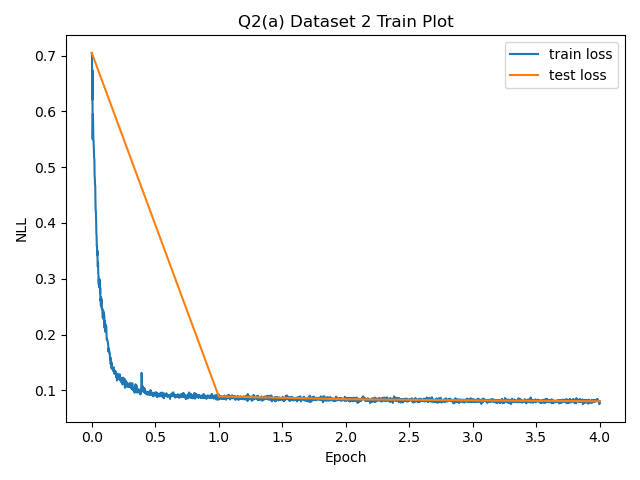
\includegraphics[width=\textwidth]{figures/q2_a_dset2_train_plot.png}
        \caption{Dataset 2: Training curve}
    \end{subfigure}
    \hspace{0.2in}
    \begin{subfigure}{0.45\textwidth}
        \centering
        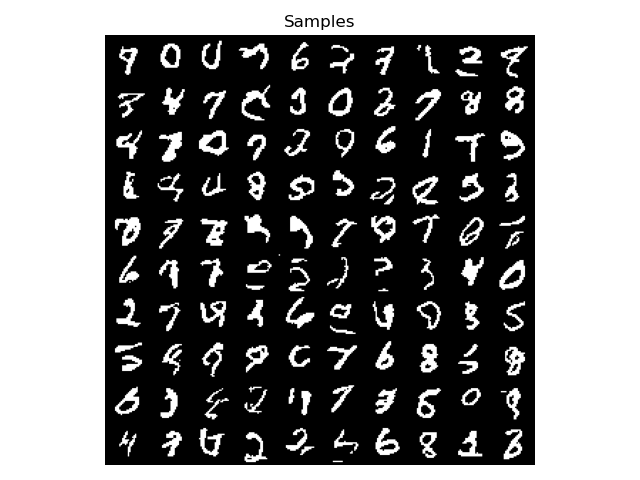
\includegraphics[width=\textwidth]{figures/q2_a_dset2_samples.png}
        \caption{Dataset 2: Samples}
    \end{subfigure}
\end{figure}

\newpage

\item {\bf [15pt] PixelCNN on Colored Shapes and MNIST: Independent Color Channels} \\\\
Final test loss for dataset 1: 0.0444  nats / dim
\begin{figure}[H]
    \centering
    \begin{subfigure}{0.45\textwidth}
        \centering
        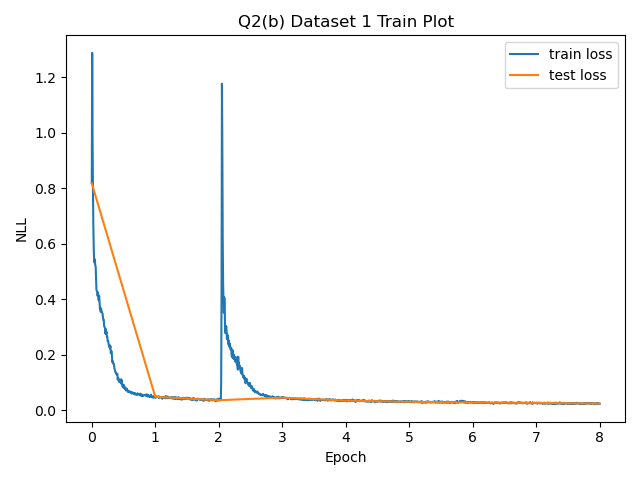
\includegraphics[width=\textwidth]{figures/q2_b_dset1_train_plot.png}
        \caption{Dataset 1: Training curve}
    \end{subfigure}
    \hspace{0.2in}
    \begin{subfigure}{0.45\textwidth}
        \centering
        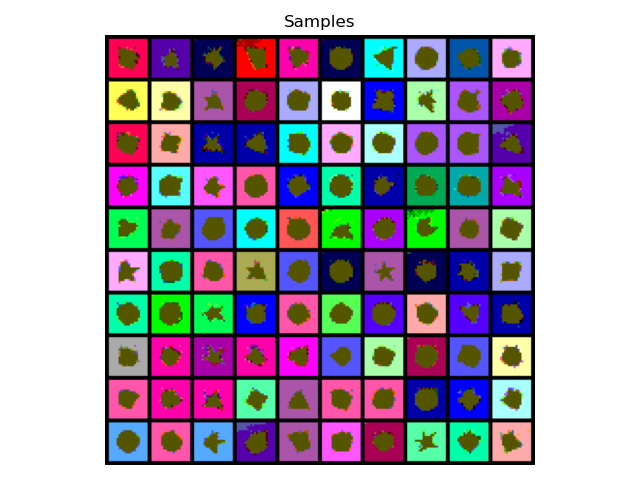
\includegraphics[width=\textwidth]{figures/q2_b_dset1_samples.png}
        \caption{Dataset 1: Samples}
    \end{subfigure}
\end{figure}
Final test loss for dataset 2: \textcolor{red}{FILL IN HERE}  nats / dim
\begin{figure}[H]
    \centering
    \begin{subfigure}{0.45\textwidth}
        \centering
        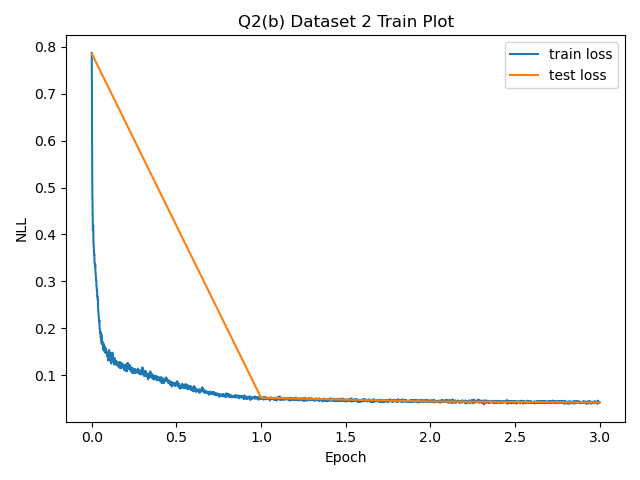
\includegraphics[width=\textwidth]{figures/q2_b_dset2_train_plot.png}
        \caption{Dataset 2: Training curve}
    \end{subfigure}
    \hspace{0.2in}
    \begin{subfigure}{0.45\textwidth}
        \centering
        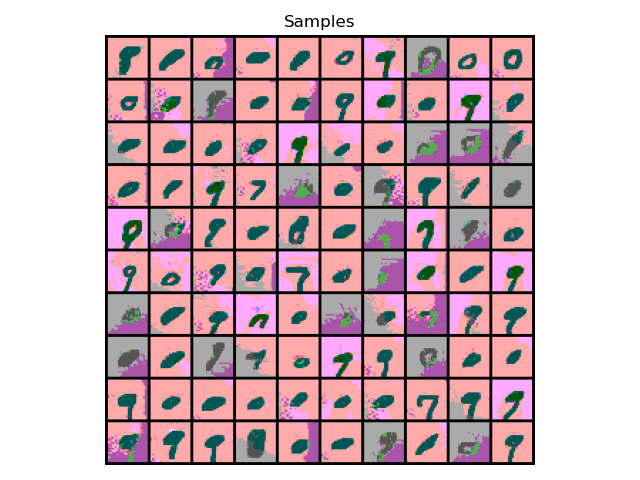
\includegraphics[width=\textwidth]{figures/q2_b_dset2_samples.png}
        \caption{Dataset 2: Samples}
    \end{subfigure}
\end{figure}
\end{enumerate}

%--------------------------------------------------------------------------------
%--------------------------------------------------------------------------------
%--------------------------------------------------------------------------------
\newpage
\noindent {\bf Question 3: Causal Transformer - iGPT}
%--------------------------------------------------------------------------------
%--------------------------------------------------------------------------------
%--------------------------------------------------------------------------------

\begin{enumerate}[(a)]
\item {\bf [15pt] Autoregressive Transformer on Shapes and MNIST} \\\\
Final test loss for dataset 1: 0.0397  nats / dim
\begin{figure}[H]
    \centering
    \begin{subfigure}{0.45\textwidth}
        \centering
        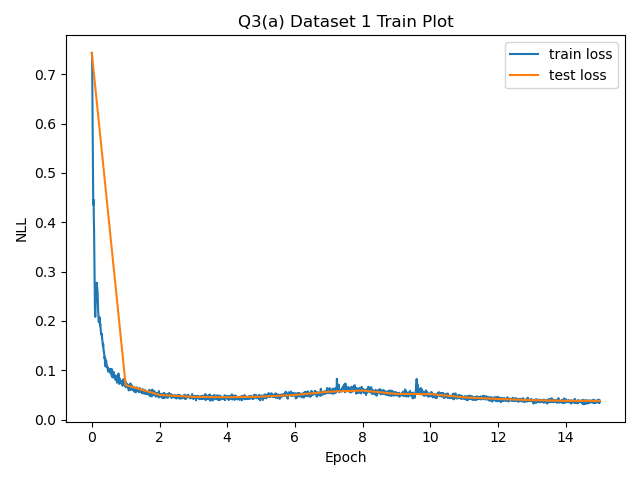
\includegraphics[width=\textwidth]{figures/q3_a_dset1_train_plot.png}
        \caption{Dataset 1: Training curve}
    \end{subfigure}
    \hspace{0.2in}
    \begin{subfigure}{0.45\textwidth}
        \centering
        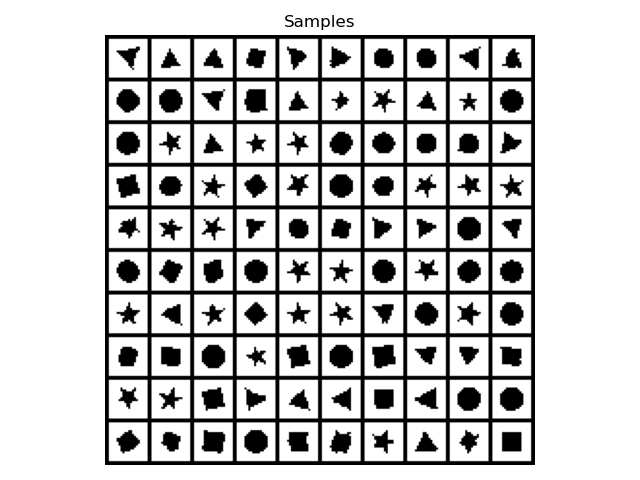
\includegraphics[width=\textwidth]{figures/q3_a_dset1_samples.png}
        \caption{Dataset 1: Samples}
    \end{subfigure}
\end{figure}
Final test loss for dataset 2: \textcolor{red}{FILL IN HERE}  nats / dim
\begin{figure}[H]
    \centering
    \begin{subfigure}{0.45\textwidth}
        \centering
        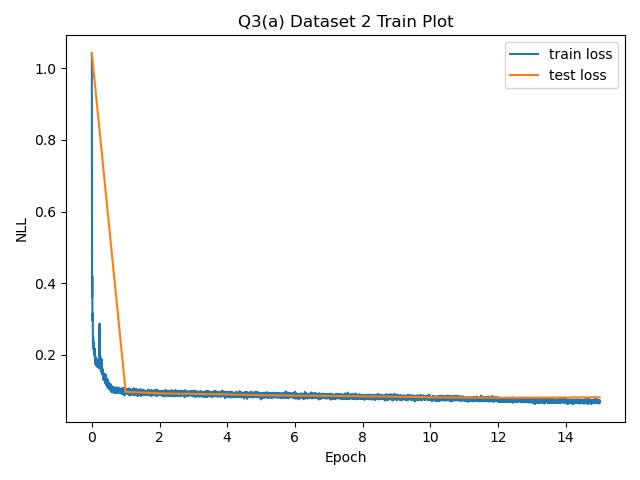
\includegraphics[width=\textwidth]{figures/q3_a_dset2_train_plot.png}
        \caption{Dataset 2: Training curve}
    \end{subfigure}
    \hspace{0.2in}
    \begin{subfigure}{0.45\textwidth}
        \centering
        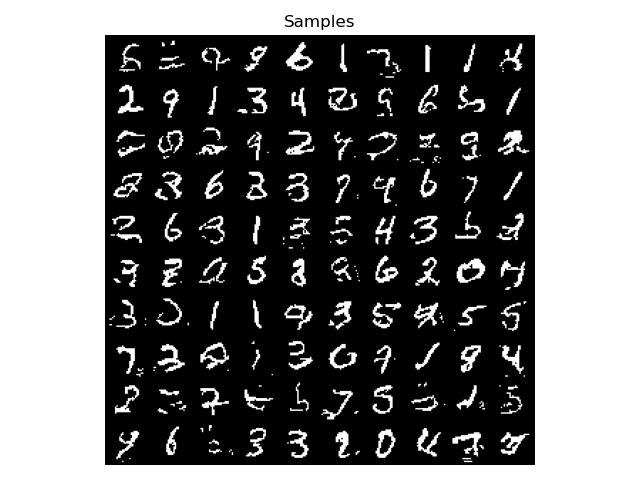
\includegraphics[width=\textwidth]{figures/q3_a_dset2_samples.png}
        \caption{Dataset 2: Samples}
    \end{subfigure}
\end{figure}

\newpage

\item {\bf [15pt] Autoregressive Transformer on Colored Shapes and MNIST} \\\\
Final test loss for dataset 1: 0.0541  nats / dim
\begin{figure}[H]
    \centering
    \begin{subfigure}{0.45\textwidth}
        \centering
        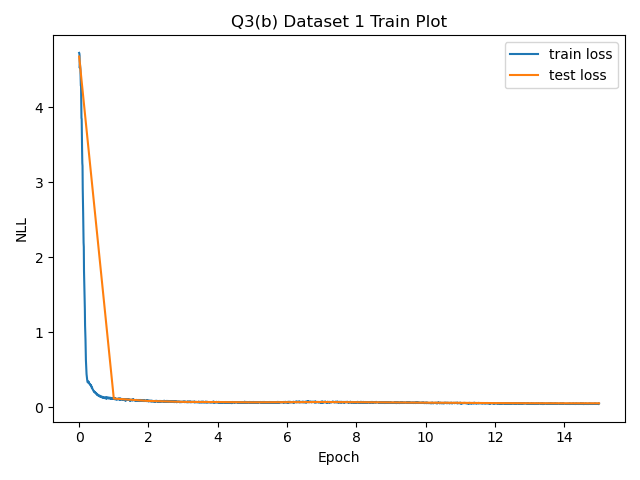
\includegraphics[width=\textwidth]{figures/q3_b_dset1_train_plot.png}
        \caption{Dataset 1: Training curve}
    \end{subfigure}
    \hspace{0.2in}
    \begin{subfigure}{0.45\textwidth}
        \centering
        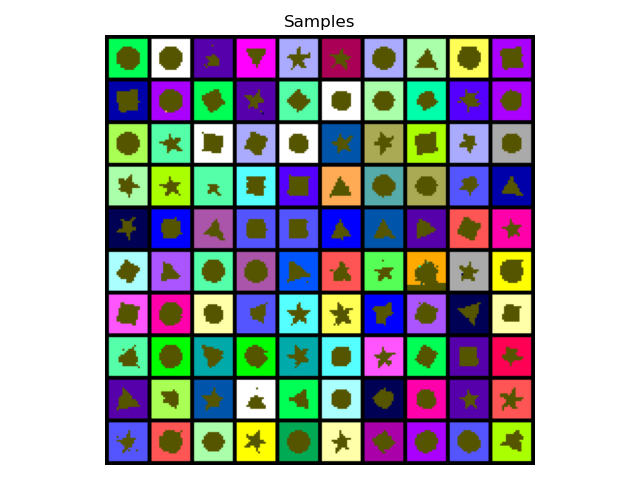
\includegraphics[width=\textwidth]{figures/q3_b_dset1_samples.png}
        \caption{Dataset 1: Samples}
    \end{subfigure}
\end{figure}
Final test loss for dataset 2: \textcolor{red}{FILL IN HERE}  nats / dim
\begin{figure}[H]
    \centering
    \begin{subfigure}{0.45\textwidth}
        \centering
        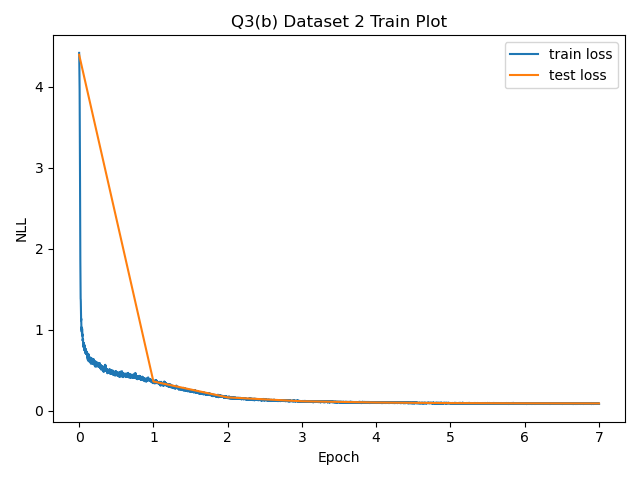
\includegraphics[width=\textwidth]{figures/q3_b_dset2_train_plot.png}
        \caption{Dataset 2: Training curve}
    \end{subfigure}
    \hspace{0.2in}
    \begin{subfigure}{0.45\textwidth}
        \centering
        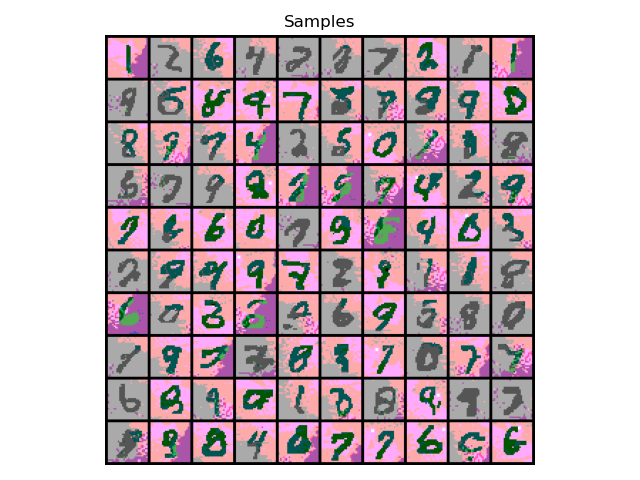
\includegraphics[width=\textwidth]{figures/q3_b_dset2_samples.png}
        \caption{Dataset 2: Samples}
    \end{subfigure}
\end{figure}

\newpage

\item {\bf [15pt] K,V Caching for Improved Inference} \\\\
\begin{figure}[H]
    \centering
    \includegraphics[width=\textwidth]{figures/q3_c_dset1_timing_plot.png}
    \caption{Dataset 2: Inference Speed}
\end{figure}

\begin{figure}[H]
    \centering
    \begin{subfigure}{0.45\textwidth}
        \centering
        \includegraphics[width=\textwidth]{figures/q3_c_no_cache_dset1_samples.png}
        \caption{Dataset 2: Samples (no caching)}
    \end{subfigure}
    \hspace{0.2in}
    \begin{subfigure}{0.45\textwidth}
        \centering
        \includegraphics[width=\textwidth]{figures/q3_c_with_cache_dset1_samples.png}
        \caption{Dataset 2: Samples (caching)}
    \end{subfigure}
\end{figure}
\end{enumerate}

%--------------------------------------------------------------------------------
%--------------------------------------------------------------------------------
%--------------------------------------------------------------------------------
\newpage
\noindent {\bf Question 4: Causal Transformer - Tokenized Images}
%--------------------------------------------------------------------------------
%--------------------------------------------------------------------------------
%--------------------------------------------------------------------------------

\begin{enumerate}[(a)]
\item {\bf [5pt] Image Quantization} \\\\
\begin{figure}[H]
    \centering
    \begin{subfigure}{0.45\textwidth}
        \centering
        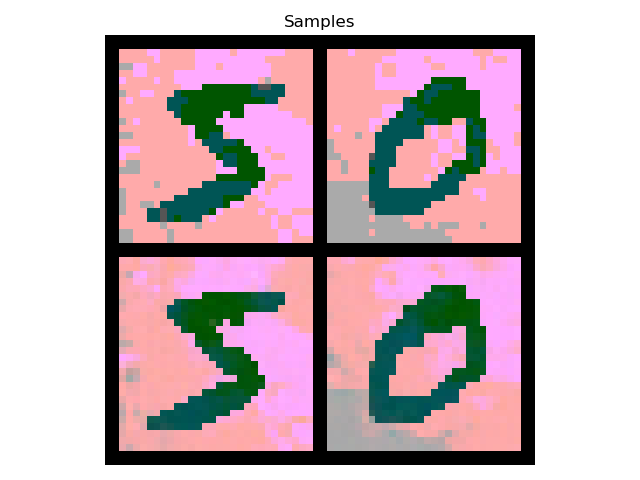
\includegraphics[width=\textwidth]{figures/q4_a_dset1_samples.png}
        \caption{Dataset 1: Quantized Examples}
    \end{subfigure}
    \hspace{0.2in}
    \begin{subfigure}{0.45\textwidth}
        \centering
        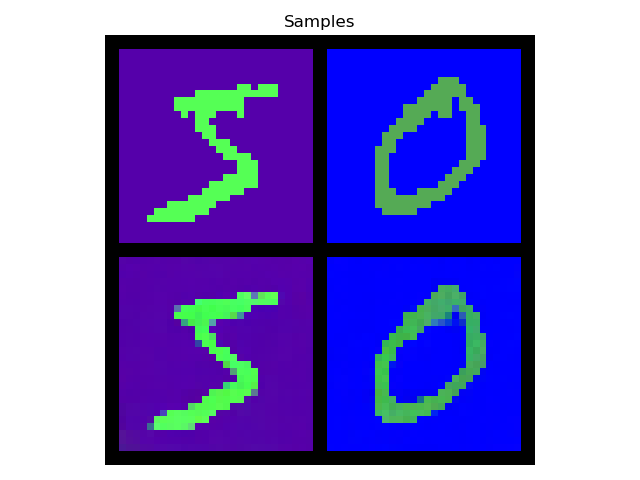
\includegraphics[width=\textwidth]{figures/q4_a_dset2_samples.png}
        \caption{Dataset 2: Quantized Examples}
    \end{subfigure} \\
\end{figure}

\item {\bf [15pt] Autoregressive Transformer on Colored Shapes and MNIST with Vector Quantization} \\\\
Final test loss for dataset 1: 3.083 nats / dim
\begin{figure}[H]
    \centering
    \begin{subfigure}{0.45\textwidth}
        \centering
        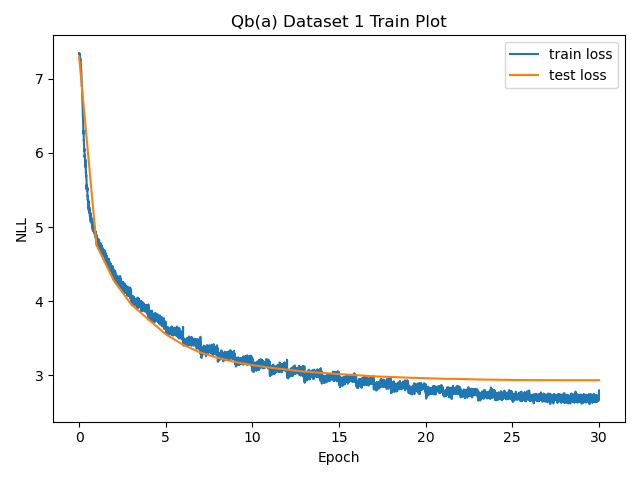
\includegraphics[width=\textwidth]{figures/q4_b_dset1_train_plot.png}
        \caption{Dataset 1: Training curve}
    \end{subfigure}
    \hspace{0.2in}
    \begin{subfigure}{0.45\textwidth}
        \centering
        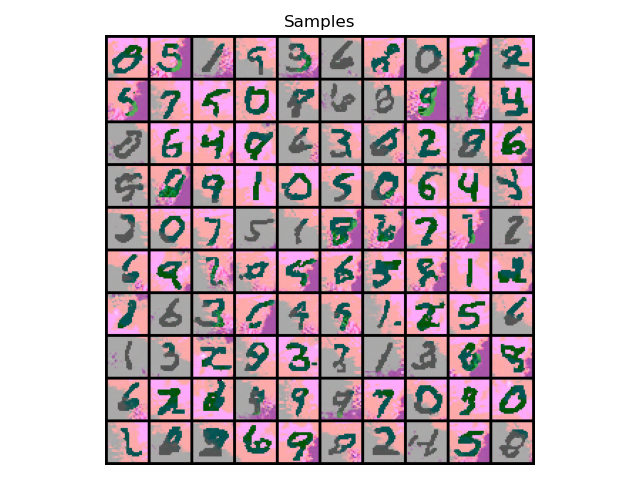
\includegraphics[width=\textwidth]{figures/q4_b_dset1_samples.png}
        \caption{Dataset 1: Samples}
    \end{subfigure}
\end{figure}
Final test loss for dataset 2: \textcolor{red}{FILL IN HERE}  nats / dim
\begin{figure}[H]
    \centering
    \begin{subfigure}{0.45\textwidth}
        \centering
        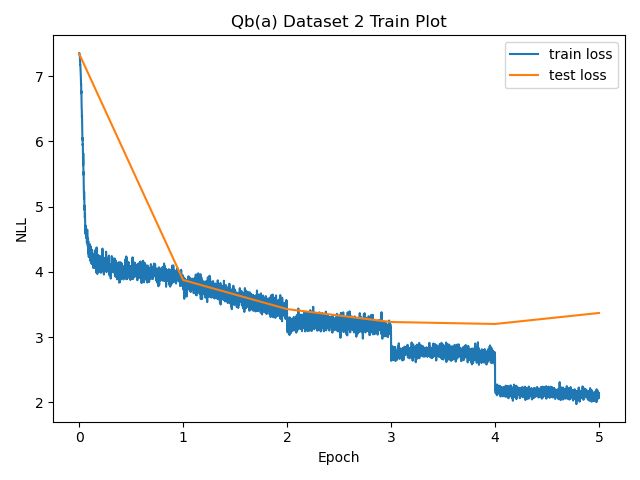
\includegraphics[width=\textwidth]{figures/q4_b_dset2_train_plot.png}
        \caption{Dataset 2: Training curve}
    \end{subfigure}
    \hspace{0.2in}
    \begin{subfigure}{0.45\textwidth}
        \centering
        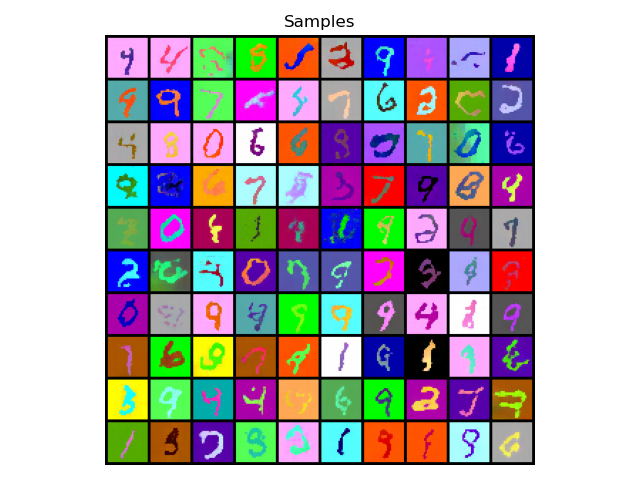
\includegraphics[width=\textwidth]{figures/q4_b_dset2_samples.png}
        \caption{Dataset 2: Samples}
    \end{subfigure}
\end{figure}

\end{enumerate}

%--------------------------------------------------------------------------------
%--------------------------------------------------------------------------------
%--------------------------------------------------------------------------------
\newpage
\noindent {\bf Question 5: Causal Transformer - Text}
%--------------------------------------------------------------------------------
%--------------------------------------------------------------------------------
%--------------------------------------------------------------------------------

\begin{enumerate}[(a)]
\item {\bf [20pt] Modeling Text} \\\\
Final test loss: \textcolor{red}{FILL IN HERE}  nats / dim
\begin{figure}[H]
    \centering
\end{figure}

\begin{figure}[H]
    \centering
\end{figure}

\begin{figure}[H]
    \centering
    \begin{subfigure}{0.3\textwidth}
        \centering
        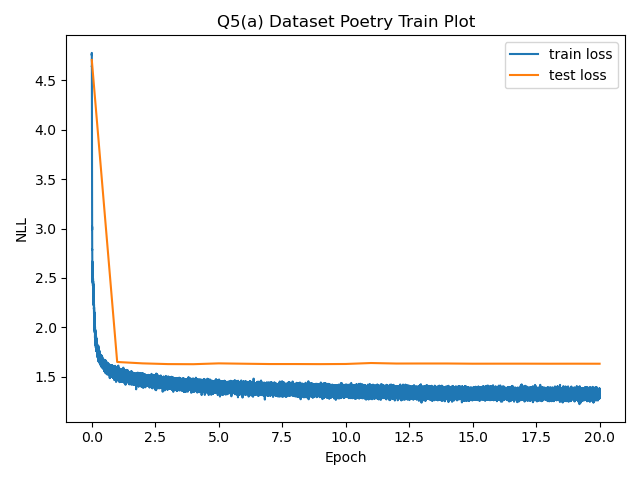
\includegraphics[width=\textwidth]{figures/q5_a_train_plot.png}
        \caption{Training curve}
    \end{subfigure}
    \hspace{0.2in}
    \begin{subfigure}{0.65\textwidth}
        \centering
        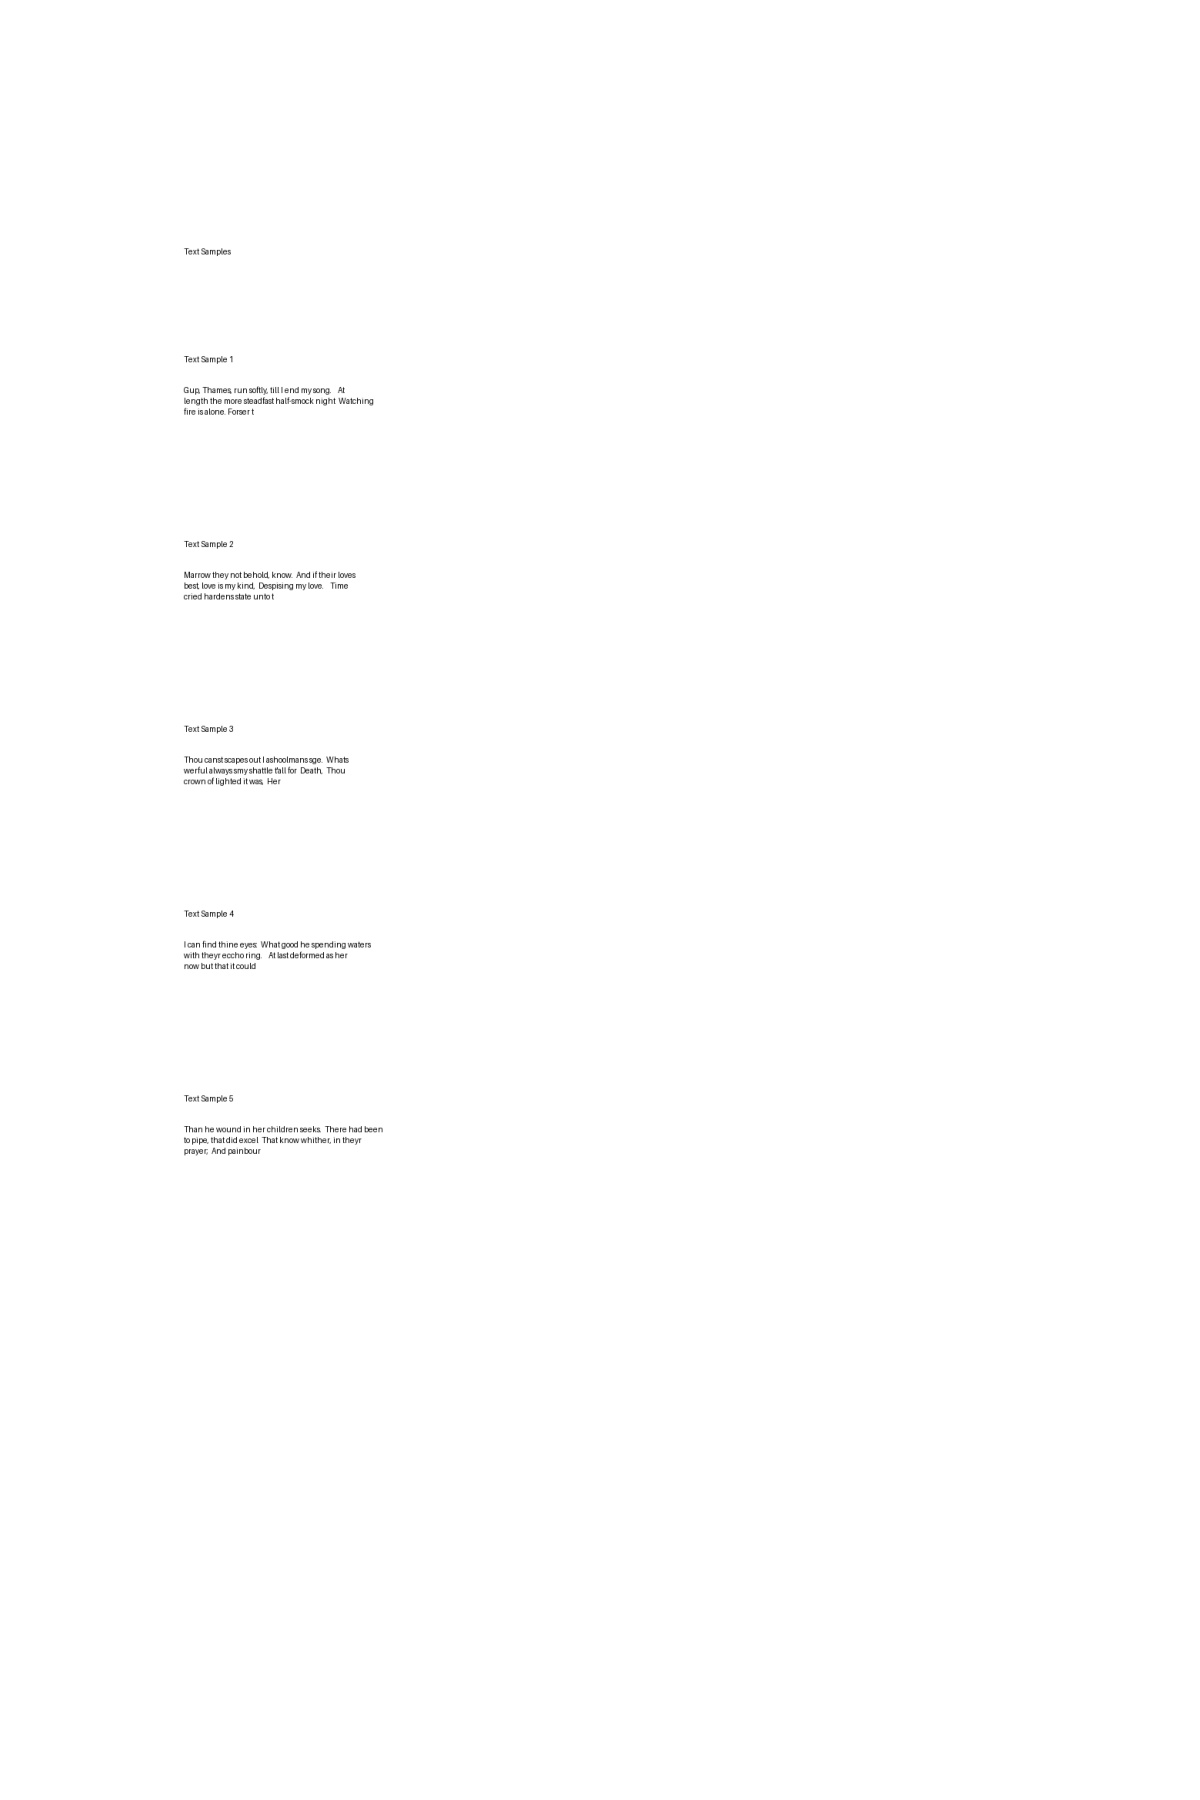
\includegraphics[width=\textwidth]{figures/q5_a_samples.png}
        \caption{Text samples}
    \end{subfigure}
\end{figure}

\end{enumerate}

%--------------------------------------------------------------------------------
%--------------------------------------------------------------------------------
%--------------------------------------------------------------------------------
\newpage
\noindent {\bf Question 6: Causal Transformer - Multimodal}
%--------------------------------------------------------------------------------
%--------------------------------------------------------------------------------
%--------------------------------------------------------------------------------

\begin{enumerate}[(a)]
\item {\bf [20pt] Multimodal Text and Image Generation} \\\\
Final test loss: \textcolor{red}{FILL IN HERE}  nats / dim
\begin{figure}[H]
    \centering
    \begin{subfigure}{0.45\textwidth}
        \centering
        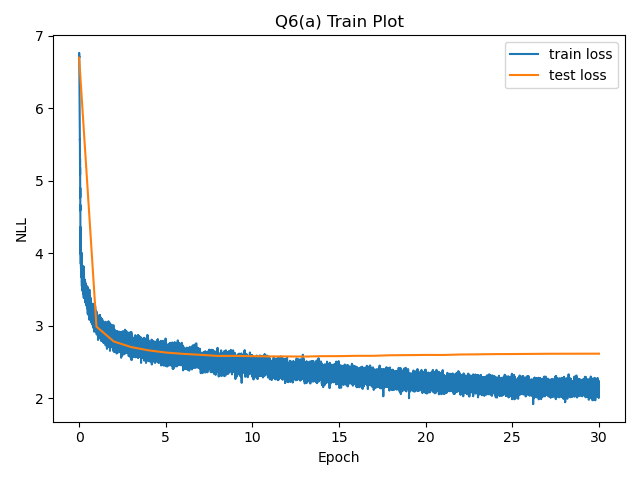
\includegraphics[width=\textwidth]{figures/q6_a_train_plot.png}
        \caption{Training curve}
    \end{subfigure}
    \hspace{0.2in}
    \begin{subfigure}{0.45\textwidth}
        \centering
        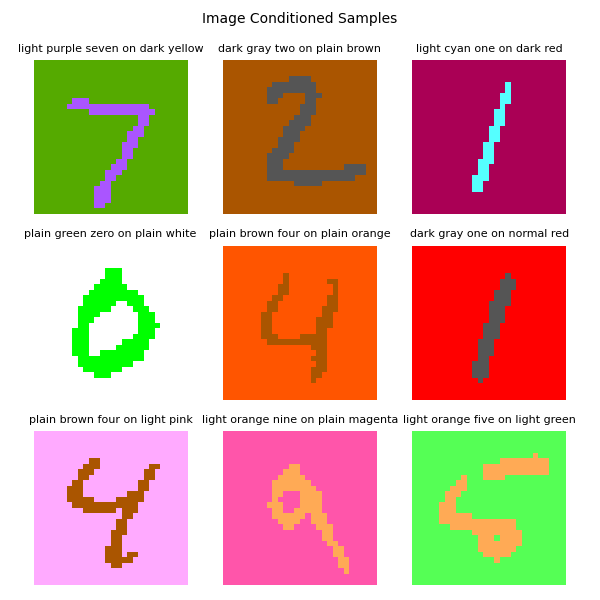
\includegraphics[width=\textwidth]{figures/q6_a_samples_img_conditioned.png}
        \caption{Image conditioned samples}
    \end{subfigure} \\
    \begin{subfigure}{0.45\textwidth}
        \centering
        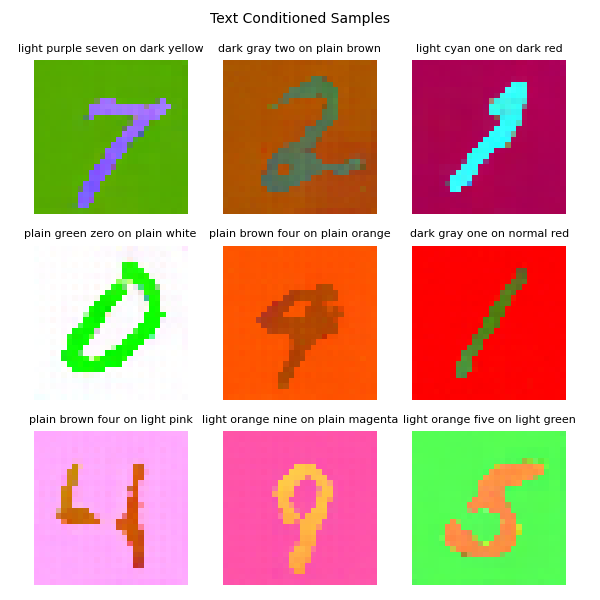
\includegraphics[width=\textwidth]{figures/q6_a_samples_text_conditioned.png}
        \caption{Text conditioned samples}
    \end{subfigure}
    \hspace{0.2in}
    \begin{subfigure}{0.45\textwidth}
        \centering
        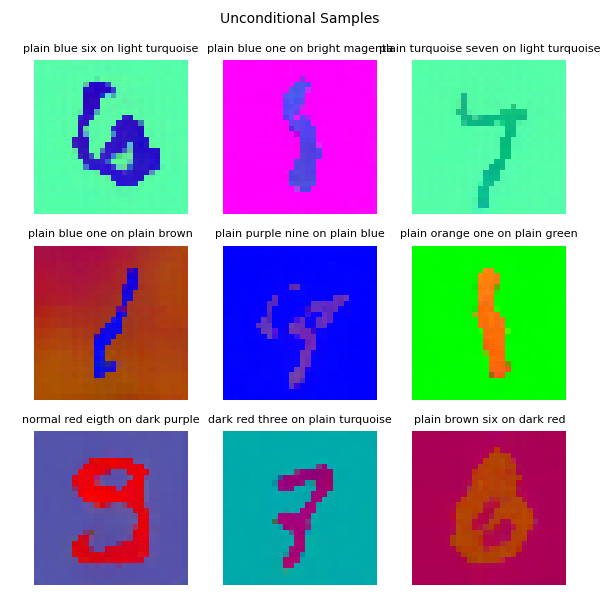
\includegraphics[width=\textwidth]{figures/q6_a_samples_unconditional.png}
        \caption{Unconditional samples}
    \end{subfigure}
\end{figure}

\end{enumerate}

\end{document}
